%!TEX root = ../crimson_throne_book_main.tex
% 2015-01-03
The companions want to explore the sunken {\itshape Delivery} further and make their way through the hatch into its cargo hold. Swimming inside they see they are not alone: \hyperref[fig:Examining-the-wreck-in-Curse-of-the-Crimson-Throne-504554608]{ a giant octopus moves in to attack } . Quint throws a  {\itshape cacophonous call} on the bottom dweller, nauseating it and forcing it to retreat in the galley. Slowly the heroes swim towards the door, but before Sjo can close it, Balian sneaks through and swings his greatsword at the large creature. Hampered by the water, his hit loses much of its strength. Puk stabs at it as well, but as the octopus has taken up position in the corner, there is no way for him to hit its vulnerable spots, so his cuts are only minor nicks. It seems like both heavy hitters have lost their advantage in this underwater environment. When Quint's spell is about to end, the bard tries to renew it, but this time his magic is resisted and the sea creature regains control of its actions. Its tentacles lash out and all the companions suddenly find themselves in the awkward grasp of rubbery arms. Balian has to drop his blade and pulls out a simple dagger to cut at his opponent. Sjo does the same, but finds it hard to score a hit. Quint, who is usually the least effective melee fighter, is all of sudden the biggest threat as his  {\itshape short sword of frost} pierces one of the tentacles, rendering it useless. The iron embrace of the octopus's arms slowly squeezes the life out of the heroes as they try to fight themselves free. Although they manage to cut off more tentacles, the crushing arms take their toll and both Sjo and Balian lose consciousness. Puk and Quint are near to the end as well: the halfling lashes about furiously with his small swords, scoring some extra scratches, but Quint saves the day by striking the final blow. \\

\begin{figure}[h]
	\centering
	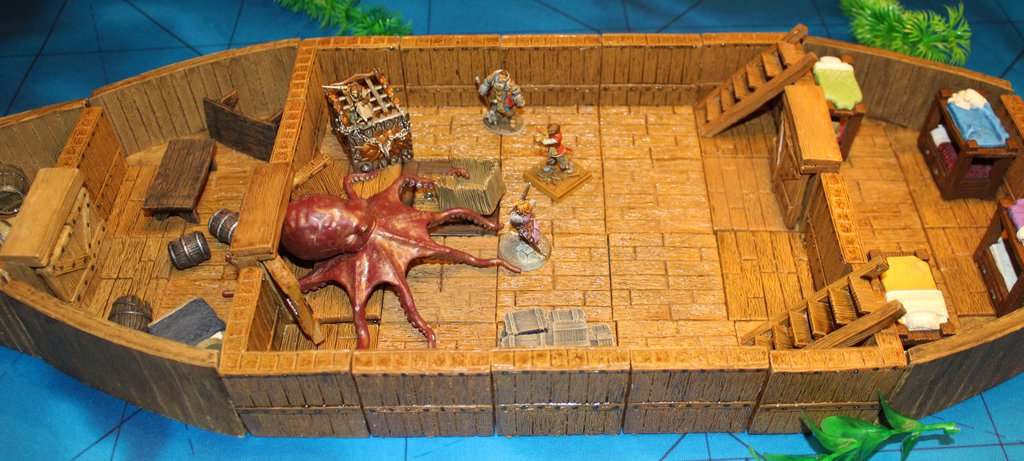
\includegraphics[width=0.39\textwidth]{images/Examining-the-wreck-in-Curse-of-the-Crimson-Throne-504554608.jpg}
	\caption{Examining the wreck in Curse of the Crimson Throne}
	\label{fig:Examining-the-wreck-in-Curse-of-the-Crimson-Throne-504554608}
\end{figure}

The companions take a few moments to heal up, before searching the cargo. There are over half a dozen big cages, the doors of which have all been opened. Each of these holds a number of dead rats, who did not die from drowning, but rather from the plague. In the lower hold the companions discover more opened cages, as well as the drowned body of a man who has an amulet of Urgathoa around his neck. There is also a ballista in here, that was used to fire the heavy shaft through the hull which caused the vessel to take on water and sink.\\

The companions return to the harbor, dry up and head to the citadel to report to Field Marshal Cressida Kroft. She encourages the heroes to examine the location marked on the map: the abandoned Porphyria manor {\itshape Lost End} . She will make a document to authorize her special task force, so the companions do not run into trouble again because they cannot prove they are working for the city. She asks them to make preparations and return tomorrow to pick up the document. The companions spend the rest of the day getting ready for their trip. They also make sure that Tayce and Brienna have enough food to get through the next couple of days without having to leave their house and risk exposure to the plague. They do the same for Madam Nesia and the children in the villa.\\

Quint also dives into the villa's library and finds more information on {\itshape Lost End} . The country house was commissioned by Lord Chadris I of House Porphyria. This nobleman was one of the wealthiest and most prominent businessmen and aristocrats in the city in his day. He was also the direct competitor of Eodred I, who was crowned the first king of Korvosa, much to Porphyria's discontent. One of Chadris's wilder business ideas was to buy up the desolate lands on the south coast of the Bay of Korvosa and try to establish a harbor there. He never got past one small landing stage in a cave, somewhere in the fierce cliffs that line the south edge of the Bay and a large manor on top of the rocks. The waters proved too treacherous to allow for any decent harbor activity and the political struggle for power in Korvosa consumed too much of his attention, so Chadris abandoned his plans to develop the area further. The manor became the Porphyria holiday house, although it found a more permanent resident in Lady Ulrika, the wife of Chadris' son, Chadris II, and mother to Chadris III, who briefly made it to the throne of Korvosa, becoming its worst and most unpopular king to date. Lady Ulrika reportedly resided in the manor for health reasons, but the truth was that she was insane and her family locked her away in the country house to avoid embarrassment in the higher circles of the city. Since the fall of the Prophyria's, at the end of Chadris's mad reign, and their banishment to Cheliax in 4667, the manor has stood empty. Since it is the last day of the month, Sjo pays a visit to the tax office and declares what the party made in the last month. Taxes amount to 4,819 gold sails, due to be paid over the next month.\\

That night Balian and Quint are awakened from their sleep by cries from Nesia's room. The girl is having a bad dream. Balian carefully wakes her up and tries to calm her down. She says she had a nightmare in which she saw the shadow of a robust man standing in a doorway. He said something to her and then closed the door, after which blood started dripping from the ceiling, slowly filling the room. As Nesia is quite shaken, Balian offers to sleep in the extra bed to watch over her.\\

